\chapter*{Introduction}
\addcontentsline{toc}{chapter}{Introduction} 

\setcounter{figure}{0}
\renewcommand{\thefigure}{I.\arabic{figure}}

The Spatial Ecosystem And POpulation DYnamics Model (SEAPODYM) is being continuously enhanced to provide a general framework allowing integration of biological and ecological knowledge of migratory species, primarily tunas and potentially other oceanic top predator species, within a comprehensive description of the pelagic ecosystem. It includes detailed relationships between the population dynamics and basic biological and ecological functions, a realistic representation of the vertical oceanic habitat in terms of both physical and foraging conditions. The forage fields are predicted by a separate model in which various mid-trophic level organisms (micronekton) are classified by their diel migration pattern, and the spatiotemporal transfer of energy from oceanic primary productivity to the micronekton is described using an allometric scaling equation and passive transport of the biomass with oceanic water masses. The environmental variables that drive fish dynamics (temperature, currents, oxygen and primary production) are predicted by coupled physical--biogeochemical models. The model also includes a rigorous mathematical parameter estimation procedure using available catch and size frequency data. Because the model includes detailed representation of the biophysical environment of the species, the complete spatially explicit population dynamics can be described with a small number of parameters. In return, such a model depends strongly on the quality of environmental forcing variables. \\

When considering the definition of an ecosystem, that is, how assemblages of species are organised in space and time, and how they interact with each other and the physical environment, modelling the ocean pelagic ecosystem is obviously a challenge that requires drastic simplifications. These simplifications need to be considered carefully alongside the level of observations and knowledge that we have for each component of the system, to make sure that the model can be properly parametrised and can adequately describe observed processes. In addition, the model is focusing on the population dynamics and the fisheries of exploited species, as there is a special interest to provide a new generation of modelling tools for the management of these species, taking into account not only the impact of the fisheries but also the natural fluctuations of the populations in their climate-driven ecosystems. Top predators in the marine pelagic ecosystem are essentially opportunistic omnivorous predators. Their diets reflect both the faunal assemblage of the components of the ecosystem that they explore and their aptitude to capture prey species during different periods of the day (i.e., daytime, night-time and twilight hours). It seems that most of them are in the upper layer during the night. But high sensory specialisation (e.g., olfaction in sharks, vision in bigeye tuna, swordfish and cephalopods, and echolocation in marine mammals), and morphological and physiological adaptations (e.g., thermoregulation) allow them also to exploit the darker and colder, deeper layers. The three-layer ocean definition used for the mid-trophic (forage) species seems to match particularly well with the known vertical behaviour of large predators (Figure~\ref{Predators_3layers}). \\


\begin{figure}[H]  
	\centering
		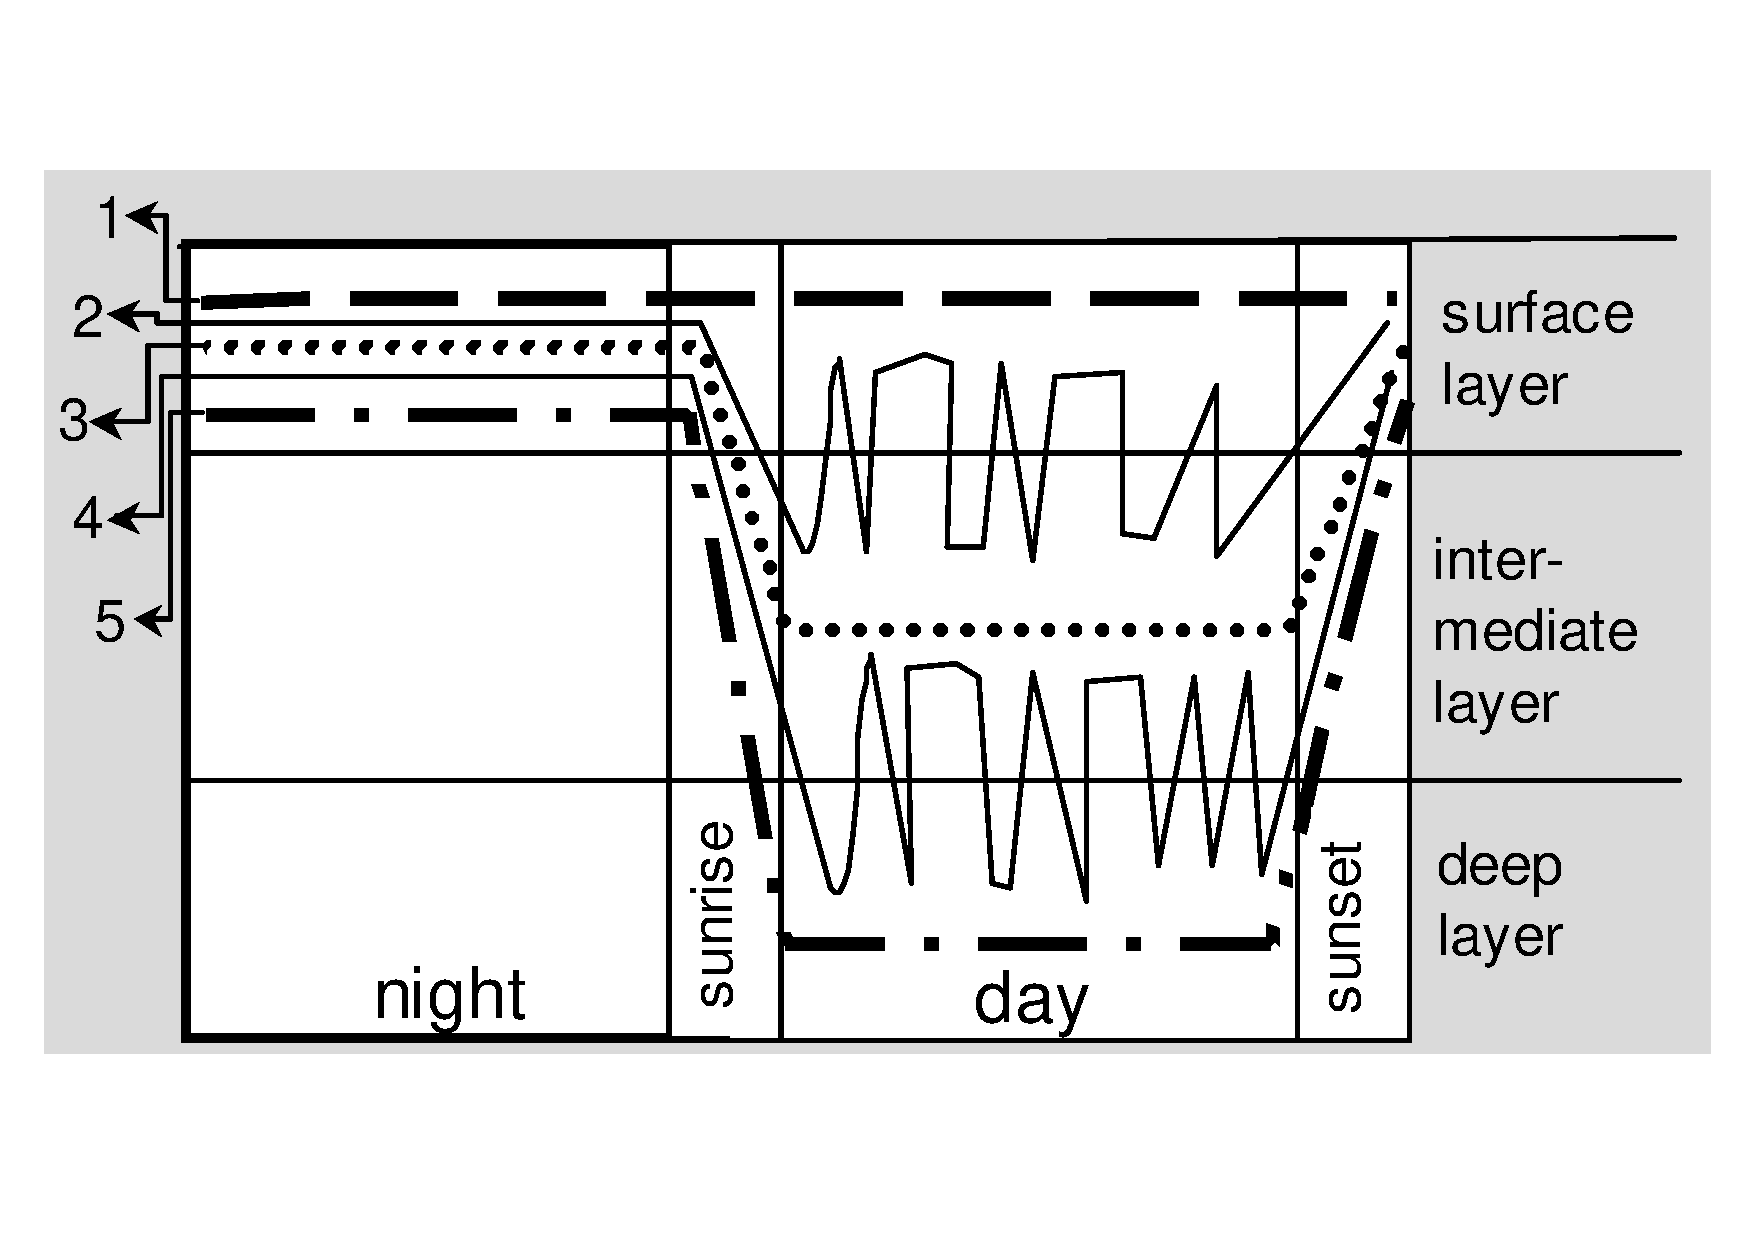
\includegraphics[width=0.95\textwidth]{intro/figs/Fig_3layersPredators}
	\caption{Five typical vertical movement behaviours simulated using a three-layer and two-type-of-prey pelagic system (adapted from Dagorn et al. 2000): 1, epipelagic predators (e.g., skipjack tuna, marlins and sailfish); 2, predators moving between the surface and intermediate layers during the day (e.g., yellowfin tuna); 3, predators mainly in the intermediate layer during the day (e.g., albacore tuna); 4, predators moving between deep and intermediate layers during the day (e.g., blue shark); 5, predators mainly in the deep layer during the day (e.g., bigeye tuna and swordfish).}
	\label{Predators_3layers}
\end{figure}

Large pelagic predators are often exploited species for which there is detailed knowledge on biology, physiology, population structure and fisheries data. Describing the spatial dynamics of these fish populations at oceanic scales is of paramount importance for fisheries management, so as to understand and predict the consequences of fishing, climate change and changes in fishery management regulations. Many spatially explicit models have been developed for fish populations; however, most of them are Lagrangian models considering only passive movements of small fish or early life stage individuals transported by currents \citep*[see, e.g.,][]{DeAngelis, Rossi, Popova, Ramesh, vanSebille}. Parametrisation of Lagrangian models can only be done by manual calibration, using empirically derived parameter values or relying on estimates from external models \citep*[as in, e.g.,][]{Scutt}. Advection-diffusion-reaction (ADR) equations were suggested by many mathematical ecologists as an elegant solution to deal with complex spatio-temporal patterns arising from animal behaviour \citep*[see, e.g.,][]{Keller-Segel,Okubo80, Okubo-Levin, Murray, Grunbaum98, Grunbaum99, Flierl, Tyutyunov, TT, Berezovskaya,Petrovskii}. While ADR equations are unsuitable for low-abundance populations sparsely distributed in space, they provide a very convenient framework for modelling spatial dynamics of migratory species that occupy vast oceanic regions and may create low- and high-density concentrations. The movement dynamics within ADR equations are governed by the distribution of stimuli attracting or repulsing the population density. This classical approach has been thoroughly studied in theoretical movement ecology, widely used in various modelling applications and its interconnections with individual movements are well understood \citep{Okubo77, Okubo80, Grunbaum94, Grunbaum98, Grunbaum99,  Flierl, Turchin, Faugeras2007, Tyutyunov2013, TT}. 

The advantages of using ADR equations can be summarised as follows. While predicting the trajectory of a single individual is impossible due to the stochastic component of its movement, the evolution of density distributions of a large number of individuals can be effectively predicted in a continuous advection--diffusion framework \citep{Grunbaum99, Flierl, Tyutyunov}. In addition, explicitly modelling movement not only leads to a reduced number of model parameters and simplified local (in every position in space) functional responses \citep*[e.g.,][]{Arditi, TT}, but also allows considering simple aggregated statistics (e.g., mean squared step length) in model parametrisations \citep{Grunbaum98}. Moreover, incorporating biological-physical interactions by accounting for the impact of temporal and spatial environmental variability on population dynamics and thus reducing the number of model parameters is more straightforward in ADR equations \citep*[e.g.,][]{Grunbaum98, Flierl} than in classical, spatially aggregated stock assessment models operating in large management regions \citep{Punt}. In exchange for their parsimony, spatially explicit dynamic models applied to full-life-cycle fish population dynamics have higher dimensionality. The latter represents the cost for being more realistic models.\\

Being continuous, ADR equations allow implementation of quantitative methods to estimate model parameters from available observations \citep{Sibert, Senina08}. Nevertheless, before applying these models to solve fishery management problems, we need to be confident in the reliability of model predictions. Hence, we need to work on developing the dynamic model, providing adequate descriptions of observed phenomena, and improving the model structure, allowing quantitative dynamics, under the tight coupling of the model predictions to observations. \\

The SEAPODYM modelling approach for top predator population dynamics has greatly benefited from the work undertaken by \citet{Sibert} on implementation of continuous ADR equations to describe movement dynamics and estimate movement and mortality rates of tagged skipjack and yellowfin tunas \citep*[see also][]{Sibert-Fournier}. SEAPODYM has been continuously evolving since the initial development of a single-cohort tuna population model presented in \citet{Bertignac}. A few years later \citet{Lehodey2001} proposed a coupled predator--prey model with the model for tuna forage. In the study of \citet{Lehodey2003}, discrete-type age structured equations were added to the numerical solver of continuous ADR equations. The first fully parametrised and fully operational SEAPODYM model was presented in \citet{Lehodey2008}, and with an added parameter estimation method in \citet{Senina08}. The general scheme of the model and parameter estimation approach is shown in Figure~\ref{model_scheme}. \\

\begin{figure}[htbp]
	\centering
	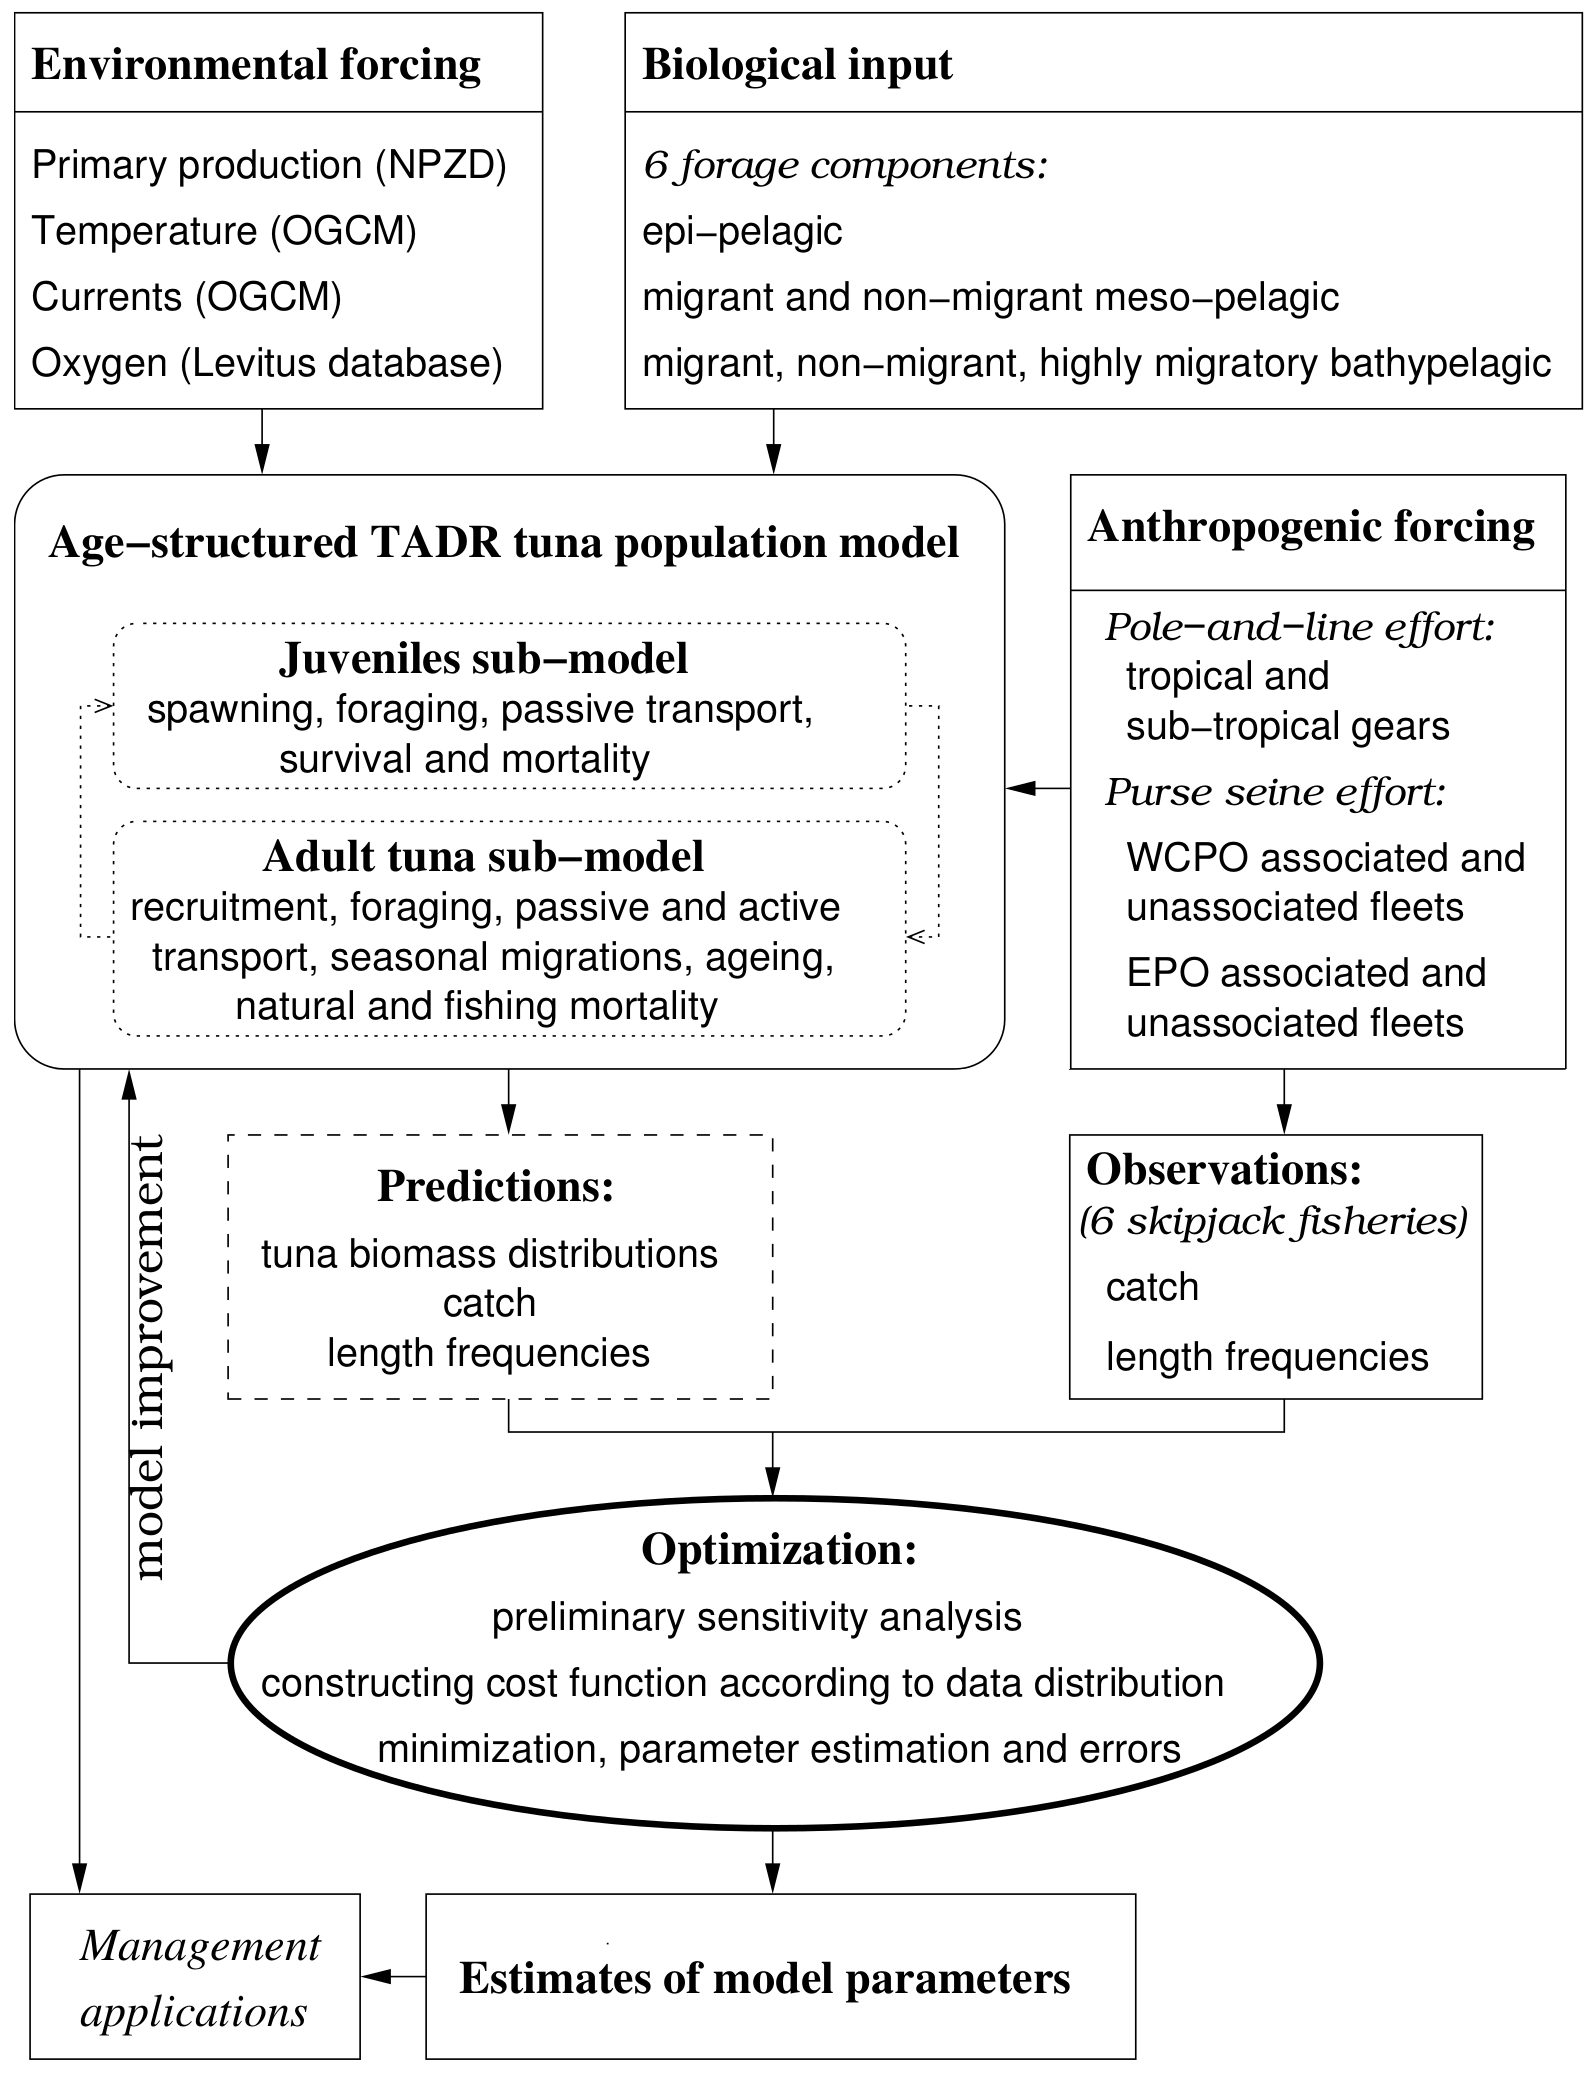
\includegraphics[width=0.85\textwidth]{intro/figs/fig-scheme-old}
	\caption{General scheme of the model with optimization approach \citep[from][]{Senina08}.} 
	\label{model_scheme}
\end{figure}

The current model version is based on a continuous ADR equation with an ageing term, and is fully described in \citet{Senina20a,Senina20b}. The SEAPODYM modelling framework now includes several models, and allows, besides the full population dynamics model, computing and estimating the parameters of spawning and feeding habitats, modelling movement dynamics of tagged cohorts, and integrating tagging data to inform movement rates of modelled fish at different ages/sizes. The model can be now be parametrised through integration of industrial fisheries data and conventional as well as archival tagging data, and optimization is carried out using the maximum likelihood estimation approach. The implementation of adjoint code allows an exact, analytical evaluation of the likelihood gradient to be obtained. The approach to select the ``best parameter estimate'' is based on a series of computer experiments in order to i) determine model sensitivity with respect to variable parameters and, hence, investigate their observability; ii) estimate observable parameters and their errors; iii) justify the reliability of found solutions; iv) validate the parametrisation with independent information; and v) compute the errors of parameter estimates. \\

The continuous improvements in the model structure, the implementation of the numerical model coupled with the quantitative methods of parameter estimation allowed numerous model applications to different pelagic species such as Pacific skipjack tuna \citep{Lehodey2013,Senina20b}, Pacific yellowfin tuna \citep{Senina2015}, Pacific bigeye tuna \citep{Senina2021}, Atlantic albacore tuna \citep{Dragon2015,Senina20a}, South Pacific albacore tuna \citep{Lehodey2015,Senina20a}, Chilean jack mackerel \citep{Dragon2017} and Pacific swordfish \citep{Abecassis}. Informing model parameters through integration of various types of data for different migratory species thus showed that such models have the capacity to provide valid quantitative predictions of the species population dynamics, and can be used in the development of management strategies \citep{Sibert2012} and in investigating the climate change impacts \citep{Lehodey2010,Lehodey2013,Lehodey2015,Bell}. All examples of applications and related projects can be found in the dedicated websites (\url{www.seapodym.eu}; \url{www.spc.int/ofp/seapodym}).\\

This reference manual for the SEAPODYM-MASS model is constructed as follows. {\hypersetup{linkcolor=black} Chapter 1, {\bfseries ``\nameref{ch:model}}"} is devoted to the mathematical model and the dynamic processes it describes. It also details the underlying biological mechanisms behind the definitions of spawning and feeding habitats. {\hypersetup{linkcolor=black} Chapter 2, {\bfseries ``\nameref{ch:numerics}}"} describes the discretisation of model dimensions, the numerical model that is the approximation of the continuous ADR equations with an ageing term, its integration with alternating-direction implicit (ADI) method and the general algorithm implementation within the main time and age loop. {\hypersetup{linkcolor=black} Chapter 3, {\bfseries ``\nameref{ch:configurations}}"} provides detailed documentation on how to run the model simulation with predefined configurations. The input and output data files are also described in this chapter. {\hypersetup{linkcolor=black} Chapter 4, {\bfseries ``\nameref{ch:parametrisation}}"} reviews the methods to build up quantitative models. This final chapter is intended for advanced use of the model, providing the methods for the model application to the new species.

\setcounter{figure}{0}
\renewcommand{\thefigure}{\arabic{chapter}.\arabic{figure}}


\addcontentsline{toc}{section}{References}

%\reftitle{References}

\begin{thebibliography}{999}
%\bibitem[Author1(year)]{ref-journal}
%Author~1, T. The title of the cited article. {\em Journal Abbreviation} {\bf 2008}, {\em 10}, 142--149.
%% Reference 2
%\bibitem[Author2(year)]{ref-book1}
%Author~2, L. The title of the cited contribution. In {\em The Book Title}; Editor1, F., Editor2, A., Eds.; Publishing House: City, Country, 2007; pp. 32--58.
%% Reference 3
%\bibitem[Author3(year)]{ref-book2}
%Author 1, A.; Author 2, B. \textit{Book Title}, 3rd ed.; Publisher: Publisher Location, Country, 2008; pp. 154--196.
%% Reference 4
%\bibitem[Author4(year)]{ref-unpublish}
%Author 1, A.B.; Author 2, C. Title of Unpublished Work. \textit{Abbreviated Journal Name} stage of publication (under review; accepted; in~press).
%% Reference 5
%\bibitem[Author5(year)]{ref-communication}
%Author 1, A.B. (University, City, State, Country); Author 2, C. (Institute, City, State, Country). Personal communication, 2012.
%% Reference 6
%\bibitem[Author6(year)]{ref-proceeding}
%Author 1, A.B.; Author 2, C.D.; Author 3, E.F. Title of Presentation. In Title of the Collected Work (if available), Proceedings of the Name of the Conference, Location of Conference, Country, Date of Conference; Editor 1, Editor 2, Eds. (if available); Publisher: City, Country, Year (if available); Abstract Number (optional), Pagination (optional).

\bibitem[Autodif User's Manual, 2021]{Autodif} AUTODIF: A C ++ Array Language Extension with Automatic Differentiation For Use in Nonlinear Modeling and Statistics. \url{https://github.com/admb-project/admb/releases/download/admb-12.3/autodif-12.3.pdf} 

\bibitem [Bard, 1974] {Bard} 
Bard, Y. Nonlinear parameter estimation. Academic Press: New York, 1974.

\bibitem [Griewank and Corliss, 1991] {Griewank} 
Griewank, A.,  Corliss, G.F.  Automatic differentiation of algorithms: theory, implementation, and application. SIAM: Philadelphia, 1991.

\bibitem[Hampton and Fournier, 2001]{Hampton-Fournier}Hampton, J., and Fournier, D.A. 2001. A spatially disaggregated, length-based, age-structured population model of yellowfin tuna (Thunnus albacares) in the western and central Pacific Ocean. Mar. Freshw. Res. 52: 937–963. \url{https://doi.org/10.1071/MF01049}.

\bibitem[Fonteneau, 1996] {Fonteneau} 
Fonteneau, A. Interactions between tuna fisheries: a global review with specific examples from the Atlantic Ocean. In Status of Interactions of Pacific Tuna Fisheries in 1995. Proceedings of the Second FAO Expert Consultation on Interactions of Pacific Tuna Fisheries, Shimizu, Japan, 23–31 January 1995; R.S. Shomura, J. Majkowski, and R.F. Harman, Eds.; FAO Fisheries Technical Paper, 1996; No. 365.

%\bibitem [Langley et al., 2005]{MFCL-SKJ} Langley, A., Hampton, J., Ogura, M.  Stock assessment of skipjack tuna in the western and central Pacific Ocean. Western And Central Pacific Fisheries Commission, Scientific Committee,SA WP4). {\bf 2005}, http://wcpfc.org/sc1/pdf/SC1\_SA\_WP\_4.pdf 

\bibitem[Matear, 1995]{Matear} Matear, R. J. 1995. Parameter optimization and analysis of ecosystem models using simulated annealing: a case study at Station P.  {\em Journal of Marine Research.} {\bf 1995}, {\em 53}, 571--607. 

\bibitem[Otter Research Ltd, 1994]{Fournier} 
Otter Research Ltd. Autodif: a C++ array extension with automatic differentiation for use in nonlinear modeling and statistics. Otter Research Ltd: Nanaimo, Canada, 1994.

\bibitem[SPC Year Book, 2016] {Yearbook} Pacific Community (SPC). 2016. Tuna Fisheries Yearbook. Western and Central Pacific Fisheries Commission, Pohnpei, Federated States of Micronesia.

\bibitem[Pianosi et al., 2016]{Pianosi} 
Pianosi, F., Beven, K., Freer, J., Hall, J., Rougier, J., Stephenson, D., and Wagener, T. Sensitivity analysis of environmental models: A systematic review with practical workflow. Environ. {\em Modell. Softw.} {\bf 79}, 214–-232. \url{https://doi.org/10.1016/j.envsoft.2016.02.008}.

%continue formatting from here

\bibitem[Robinson and Lermusiaux, 2002]{Robinson} Robinson, A.R., Lermusiaux, P. F. J. 2002. Data assimilation for modeling and predicting coupled physical biological interactions in the sea. From \textit {The Sea}, Volume 12, edited by Allan R. Robinson, James J. McCarthy, and Brian J. Rothschild. John Wiley \& Sons, Inc., New York. 475-536.

\bibitem[Saltelli et al., 2008]{Saltelli} Saltelli, A., Ratto, M., Andres, T., Campolongo, F., Cariboni, J., Gatelli, D., et al. 2008. Global sensitivity analysis. The Primer. John Wiley and Sons.

\bibitem[Senina et al., 2008]{Senina08} Senina, I., Sibert, J., and Lehodey, P. 2008. Parameter estimation for basin-scale ecosystem-linked population models of large pelagic predators: Application to skipjack tuna. Prog. Oceanogr. 78: 319–335. doi:10.1016/j.pocean.2008.06.003.

%\bibitem[Senina et al., 2012]{Senina12} Senina, I., Royer, F., Lehodey, P., Hampton, J., Nicol, S., Ogura, M., et al. 2012. Integrating conventional and electronic tagging data into SEAPODYM. Pelagic Fish. Res. Prog. Univ. Hawaii Manoa Newslett. 16(1): 9–14.

\bibitem[Senina et al., 2020a]{Senina20a} Senina, I., Lehodey, P., Hampton, J. and J. Sibert. 2020a. Quantitative modelling of the spatial dynamics of South Pacific and Atlantic albacore tuna populations. \textit{Deep Sea Res. II}  175,  doi.org/10.1016/j.dsr2.2019.104667).  

\bibitem[Senina et al., 2020b]{Senina20b} Senina, I., Lehodey, P., Sibert, J. and J. Hampton. 2020b. Integrating tagging and fisheries data into a spatial population dynamics model to improve its predictive skills. \textit{Can. J. Aquat. Fish. Sci.} 77, 576–593.

\bibitem[Senina et al., 2020c]{Senina2020c} Senina, I., Lehodey, P., Nicol, S., Scutt Phillips, J., Hampton, J., 2020c. SEAPODYM: revisiting bigeye reference model with conventional tagging data. WCPFC-SC16-2020.

\bibitem[Sibert et al., 1999]{Sibert} Sibert, J.R., Hampton, J., Fournier, D.A., Bills, P.J. 1999. An advection-diffusion-reaction model for the estimation of fish movement parameters from tagging data, with application to skipjack tuna ({\it Katsuwonus pelamis}). \textit {Can. J. Fish. Aquat. Sci.} 56, 925-938. 

%\bibitem[Sibert and Hampton, 2003]{Sibert-Hampton} Sibert, J., Hampton, J. 2003. Mobility of tropical tunas and the implications for fishery management. \textit {Marine Policy} 27: 87-95.
%Procedings of the Second FAO Expert Consultation on Interactions of Pacific Ocean Tuna Fisheries, Shimizu, Japan, 23-31 January, 1995; FAO Fish. Tech. Pap. 365:402-418, Rome, 1996, 612pp. edited by R. S. Shomura, J. Majkowski, and R. F. Harman. 1996.

\bibitem[Taylor, 2001]{Taylor} Taylor, K.E. 2001. Summarizing multiple aspects of model performance in a single diagram. J. Geophys. Res. 106: 7183–7192. \url{https://doi.org/10.1029/2000JD900719}.

\bibitem[Vallino, 2000]{Vallino} Vallino, J.J. 2000. Improving marine ecisystem models: use of data assimilation and mesocosm experiments. \textit {Journal of Marine Research.} 58, 117-164.

\bibitem[Worley, 1991]{Worley} Worley, B. 1991. Experience with the forward and reverse mode of GRESS in contaminent transport modeling and other applications. In Griewank, A. and G.F. Corliss. Automatic differentiation of algorithms: theory, practice and application. SIAM, Philadelphia.

\end{thebibliography}


%%%%%%%%%%%%%%%%%%%%%%%%%%%%%%%%%%%%%%%%%%%%%%%%%%%%%%%%%%%%%%%%%%%%%%%%%%%%%%%%%%%%%%%%%%%%%%%%%%%

%%% Local Variables:
%%% TeX-master: "../Seapodym_user_manual.tex"
%%% End: